% =============================================================================
% FAECO 中文期刊版式（计算机辅助设计与图形学学报模板近似）
% 字体说明：模板要求方正书宋_GBK/方正仿宋_GBK/黑体/Times New Roman。
% 方正 GBK 字库为商业字体，需作者自行购买安装；当前以系统宋体/黑体/仿宋近似。
% 安装方正字库后，将下方 FZ 字体变量替换为对应方正字体名即可。
% =============================================================================
\documentclass[twocolumn,10pt,fontset=windows]{ctexart}

% -----------------------------------------------------------------------------
% 字体（方正 GBK 安装后替换此处）
%   正文:    \setCJKmainfont{方正书宋_GBK}
%   标题:    \setCJKsansfont{方正黑体_GBK}
%   仿宋:    \setCJKfamilyfont{fzfs}{方正仿宋_GBK}
% 当前用系统字体近似（fontset=windows: 宋体/黑体/楷体/仿宋）
% -----------------------------------------------------------------------------
\setmainfont[Path=./fonts/,Extension=.ttf,UprightFont=times,BoldFont=timesbd,ItalicFont=timesi,BoldItalicFont=timesbi]{Times New Roman}
\setCJKmainfont[Path=./fonts/,Extension=.ttf]{FZShuSong-Z01}
\setCJKsansfont[Path=./fonts/,Extension=.ttf]{SimHei}
\newCJKfontfamily\songfamily[Path=./fonts/,Extension=.ttf]{FZShuSong-Z01}
\newCJKfontfamily\fangfamily[Path=./fonts/,Extension=.ttf]{FZFangSong-Z02}
\newCJKfontfamily\heifamily[Path=./fonts/,Extension=.ttf]{SimHei}
\usepackage{amsmath,amssymb}
\usepackage{newtxmath}
\let\songti\songfamily\let\heiti\heifamily\let\fangsong\fangfamily
\usepackage{booktabs}
\usepackage{graphicx}
\usepackage{subfig}
\usepackage{float}
\usepackage{array}
\usepackage[nocompress]{cite}
\usepackage[hidelinks]{hyperref}
\usepackage{xurl}
\usepackage{algorithm}
\usepackage{algpseudocode}
\usepackage{multirow}
\usepackage{geometry}
\usepackage{placeins}
% 注意：双栏模式下 \FloatBarrier 遇到待排浮动体会退化为 \clearpage，造成栏底留白、
% 正文后移、参考文献被挤成孤儿末页。本稿正文已不再插入 \FloatBarrier（正文仅保留
% 图 2 之后一处用于约束全宽浮动体）；压页请优先调整浮动体参数，勿缩字体/行距/砍内容。
\usepackage{dblfloatfix}
\usepackage{balance}

% 版面：A4 双栏，栏宽 21.59 字符、栏间距 3 字符（以 3zw 近似）
\geometry{a4paper,left=2.0cm,right=2.0cm,top=2.1cm,bottom=2.1cm,columnsep=31.5pt}

\renewcommand{\eqref}[1]{\textup{（\ref{#1}）}}
\graphicspath{{../figures/}}
\setlength{\emergencystretch}{3em}
\Urlmuskip=0mu plus 3mu\relax
\raggedbottom
\setlength{\floatsep}{6pt plus 2pt minus 2pt}
\setlength{\textfloatsep}{8pt plus 2pt minus 2pt}
\setlength{\intextsep}{6pt plus 2pt minus 2pt}
\setlength{\dblfloatsep}{6pt plus 2pt minus 2pt}
\setlength{\dbltextfloatsep}{8pt plus 2pt minus 2pt}

% -----------------------------------------------------------------------------
% 标题层级（模板：1级11.5pt黑体 / 2级五号黑体 / 3级10pt书宋）
% -----------------------------------------------------------------------------
\ctexset{
  section = {format=\heiti\fontsize{11.5}{15}\selectfont, beforeskip=6pt, afterskip=4pt},
  subsection = {format=\heiti\fontsize{10.5}{14}\selectfont, beforeskip=5pt, afterskip=3pt},
  subsubsection = {format=\songti\fontsize{10}{13}\selectfont, beforeskip=4pt, afterskip=2pt}
}

% 图题（书宋9pt）、表题（黑体9pt）、表注/分图题（书宋8pt）
\usepackage{caption}
\DeclareCaptionFont{songti}{\songti}
\DeclareCaptionFont{heiti}{\heiti}
\captionsetup[figure]{font={songti,small},labelfont={bf},skip=3pt}
\captionsetup[table]{font={heiti,small},labelfont={bf},skip=3pt}
% subfig is not used in this manuscript; do not configure an unused subfloat caption.
\captionsetup{labelsep=space}

\begin{document}

\pagestyle{plain}

% -----------------------------------------------------------------------------
% 中文首部：标题/作者/单位/摘要/关键词/中图法分类号/DOI
\twocolumn[
\vspace*{-0.25cm}
\begin{center}
{\heiti\zihao{3} FAECO：面向预布局门级时序 ECO 的候选探索与失效刻画}\par
\vspace{6pt}
{\fangsong\zihao{4} 佟亚龙、刘畅}\par
\vspace{4pt}
{\songti\fontsize{8}{12}\selectfont（国防科技大学计算机学院，长沙 410073）}\par\vspace{2pt}
{\songti\fontsize{8}{12}\selectfont E-mail：chancews@qq.com（通信作者）}\par
\vspace{6pt}
\end{center}
\begin{flushleft}
  {\heiti\fontsize{8.5}{13}\selectfont 摘\quad 要：}{\songti\fontsize{8.5}{13}\selectfont 预布局门级时序 ECO 通过局部修改映射网表改善时序违例，但候选多、验证开销大。为此提出候选探索与失效刻画框架 FAECO：在违例路径局部逻辑上以多特征加权割生成并排序 R/G/B/JOINT 候选；将候选失效刻画为六类，作为搜索诊断与消融分析的依据；候选按轮提交：先经函数与结构检查，再由时序分析评估，最终网表另经等价性检查。在 ISCAS89、ITC-99 和 PicoRV32 上，8/8、18/19 和 2/2 个实例取得预布局理想线网 WNS 改善（PicoRV32 第三个子模块无 setup 路径，不参与改善判定），其余无退化。固定权重、20 轮迭代下，混合候选平均改善 1.07\,ns，高于仅门尺寸调整的 0.16\,ns。消融实验显示，指数滑动平均失效反馈未带来额外收益，结构重综合候选也未带来额外 WNS 改善；逻辑深度降低不等于 WNS 改善。}
\par
\vspace{4pt}
{\heiti\fontsize{8.5}{13}\selectfont 关键词：}{\songti\fontsize{8.5}{13}\selectfont 时序 ECO；局部门级修改；多特征加权割；类型化失效刻画；分层验证；预布局时序优化}\par
\vspace{2pt}
{\songti\fontsize{8.5}{13}\selectfont 中图法分类号：TP391.41}\par
\vspace{3pt}
\end{flushleft}
\vspace{2pt}
% 英文题录
\begin{center}
{\bfseries\fontsize{12.5}{16}\selectfont FAECO: Candidate Exploration and Failure Characterization for Pre-Placement Gate-Level Timing ECO}\par
\vspace{3pt}
{\normalsize Tong Yalong, Liu Chang\par}
\vspace{3pt}
{\small \itshape (College of Computer Science, National University of Defense Technology, Changsha 410073, China)}\par
\vspace{4pt}
\end{center}
\begin{flushleft}
  {\bfseries Abstract:} {\small Pre-placement gate-level timing ECO improves timing by locally modifying the mapped netlist, yet candidates are numerous and per-candidate verification is costly. FAECO is a framework for candidate exploration and failure characterization. It builds and ranks R/G/B/JOINT candidates over local logic around violating paths via a multi-feature weighted cut and a critical-path cover cut, and characterizes candidate failures into six types used for search diagnosis and ablation analysis. Candidates are committed round by round: first screened by function and structural checks, then evaluated by timing analysis, the final netlist verified by equivalence checking. On ISCAS89, ITC-99 and PicoRV32, 8/8, 18/19 and 2/2 instances achieve pre-placement ideal-net WNS improvement (the third PicoRV32 module has no setup path and is excluded), with no regression on the rest. Under fixed weights and 20 rounds, mixed candidates improve WNS by 1.07\,ns on average versus 0.16\,ns for gate sizing alone. Ablations show no extra benefit from moving-average failure feedback or structure-resynthesis candidates; lower logic depth does not imply WNS improvement.}\par
\vspace{3pt}
{\bfseries Key words:} {\small gate-level timing ECO; gate-level local modification; multi-feature weighted cut; typed failure characterization; layered verification; pre-placement timing optimization}\par
\end{flushleft}
]%


% =============================================================================
% I. 引言
% =============================================================================
\section{引言}

\subsection{背景与问题}
工程变更命令（engineering change order，ECO）按修复目标可分为功能 ECO 与时序 ECO：前者修复逻辑功能错误，后者修复时序违例。本文聚焦综合后、布局布线前的门级时序 ECO。本文将“局部门级修改”定义为在已映射网表的违例扇入锥上执行等价单元替换（结构替换）、门尺寸调整与缓冲器插入（B/G 优化）以及少量多门组合。传统时序 ECO 主要依赖缓冲器插入（buffer insertion，B）与门尺寸调整（gate sizing，G），通过改变单元驱动能力及路径负载改善最差负松弛（worst negative slack，WNS）与总负松弛（total negative slack，TNS）。在严重路径违例下，B/G 优化能力不足，其结构重映射仍受候选空间限制\cite{ho2010eco,liu2021rlsizer,chen2024aito}。

除 B/G 外，已有研究还通过技术重映射和局部逻辑补丁扩大 ECO 的结构调整空间；此类方法能够改变局部逻辑实现，但通常需要额外的功能等价验证与候选筛选。逻辑补丁构造与物理优化的协同关系直接影响功能等价验证和时序收益。

上述方法留下三个需要在公开工具链上量化的问题：第一，如何扩大深层逻辑的局部门级候选空间；第二，如何控制候选的功能、时序和物理验证成本；第三，如何对候选失效进行类型化刻画，以及这些失效信息在搜索诊断与候选控制中的作用。
\subsection{研究动机}
本文面向预布局门级时序 ECO，研究如何在违例扇入锥内构造更多局部修改候选，并利用关键路径信息安排候选评估顺序。FAECO 通过多特征加权割与关键路径覆盖割生成候选，并对验证失败的候选进行分类，以支持后续搜索控制。

实验对象为已映射到公开 SKY130 HD 标准单元库的 ISCAS89\cite{iscas89}、ITC-99\cite{itc99} 与 PicoRV32\footnote{\url{https://github.com/YosysHQ/picorv32}} 三个测试集；候选时序收益由理想线网 STA 评估，部分实验进一步采用简化 SPEF 复测，并对最终修复网表执行独立顺序 SEC 检查。

\subsection{主要贡献}
本文的主要贡献如下：

\begin{enumerate}
  \item \textbf{候选探索框架}：提出面向预布局门级时序 ECO 的候选探索框架，通过多类型局部修改候选生成与候选排序扩展搜索空间，并降低候选验证开销。在固定权重、20 轮迭代配置下，混合候选策略相较单一门尺寸调整策略取得更大的平均 WNS 改善（1.07\,ns 对 0.16\,ns）。
  \item \textbf{候选失效刻画机制}：建立候选失效刻画机制，将验证失败划分为功能与结构、边界、尺寸、时序收益、验证超时和物理复测六类（F1--F6），用于分析候选搜索瓶颈并提供参数调整依据。该机制的定位是\textbf{搜索诊断与候选控制}——为下一轮候选构造提供输入，而非独立的收敛增益来源；固定权重与自适应反馈的对照实验支持这一定位。
  \item \textbf{迭代 ECO 与分层验证流程}：构建按轮提交的门级 ECO 流程与统一数据流——每轮基于更新后的网表重新提取违例锥并生成候选，候选依次经函数与结构检查、理想线网 STA 评估和简化 SPEF 复测，最终修复网表再经独立顺序 SEC 验证。在 ISCAS89、ITC-99 和 PicoRV32 测试集上，分别有 8/8、18/19 和 2/2 个实例取得严格 WNS 改善（PicoRV32 第三个子模块无 setup 路径）。
\end{enumerate}

% =============================================================================
% II. 相关工作
% =============================================================================
\section{相关工作}

\subsection{结构重映射与逻辑补丁}
现有 ECO 方法主要涉及结构重映射、逻辑补丁构造和 B/G 物理优化等方向。

结构重映射通过替换局部单元及调整逻辑实现改善时序，部分方法结合缓冲器插入和门尺寸调整\cite{ho2010eco}，或以符号采样搜索修正点\cite{kravets2019symbolic}。FAECO 在候选生成阶段利用 Liberty 函数匹配筛选可替换单元，再进行时序评估；全局顺序等价性检查（sequential equivalence checking，SEC）作为独立验证环节。例如，\cite{ho2010eco}的备用单元分配以布线后负载为输入，FAECO 则在预布局阶段完成候选构造；\cite{kravets2019symbolic}的符号采样扩大搜索范围，并通过验证结果筛选修正点。

逻辑补丁构造通常先围绕目标修正点提取局部逻辑窗口；随后利用功能约简与反相器图（functionally reduced and-inverter graph，FRAIG）表示候选逻辑，再通过 SAT 证明筛选与原逻辑功能等价的补丁，以修复功能错误\cite{jiang2010fraig,jiang2016resource}。

后续工作进一步将资源代价纳入补丁生成，并采用 SAT 或组合等价性检查（combinational equivalence checking，CEC）进行复核\cite{jiang2016resource,zhong2024stp}。FAECO 将可计算的局部功能保持信息提前用于候选排序，并把理想线网时序测量作为独立接受信号。

当等价性验证失败时，代表性流程通常需要扩大搜索窗口或增加补丁规模重新枚举\cite{zhuo2018patch}；窗口扩展与补丁重新枚举会增加候选生成及验证开销。

B/G 物理优化近年来主要沿门尺寸调整、联合 B/G 和物理感知方向发展\cite{liu2021rlsizer,huang2025phys,chen2024aito,zhang2025buffalo}，学习驱动方法\cite{chen2024aito,zhang2025buffalo}进一步提升了其效率。这类方法主要通过调整单元驱动能力和网络负载改善时序，通常不涉及布尔功能重构；FAECO 则在已映射网表的违例扇入锥上构造多类局部候选，并利用关键路径信息对候选进行排序。

\subsection{B/G 物理优化与研究定位}
上述相关工作中的若干方法依赖商用 EDA 引擎或内部工业流程；本文选择公开的 Yosys\footnote{\url{https://yosyshq.net/yosys/}}、OpenSTA\footnote{\url{https://github.com/parallaxsw/OpenSTA}} 与 OpenROAD\cite{openroad}，在 SKY130 HD\footnote{\url{https://github.com/google/skywater-pdk}} 上实现并评估门级候选搜索。FAECO 流程覆盖映射网表、候选生成、理想线网静态时序分析（STA）和布局及全局布线寄生估计核验；顺序主实验采用构造级状态保持检查，独立的全网表 SEC 作为后续验证环节。

从应用阶段看，结构重映射与 B/G 物理优化通常用于布局后或布线阶段的物理微调，逻辑补丁构造则多在综合后、布局前执行功能修复。FAECO 面向已映射网表，将局部候选搜索与预布局时序评估结合：在已映射网表上进行局部门级修改，同时用理想线网 STA 和简化线载模型进行预布局筛选。

由于上述方法的评估依赖不同的输入与基础设施，本文不与它们进行直接的定量对比：结构重映射类方法的备用单元分配以布线后负载和备用单元布局为输入，其收益依赖实际布局信息；逻辑补丁构造类方法以功能等价性（SAT/CEC）而非 WNS 改善为接受判据，二者的评价目标不同；B/G 物理优化中的学习驱动方法需要训练环境与训练数据，而物理优化流程多依赖商用 EDA 引擎或内部工业流程，难以在公开条件下复现。本文因此采用公开工具链在统一的映射与约束条件下评估，并以候选级 STA 次数作为可复现的代价度量；比较重心落在候选空间、候选排序与验证开销三项可在公开工具链上复现的维度。各类方法与直接定量比较之间的主要障碍见表~\ref{tab:baseline_cmp}。

上述四类方法的主要侧重点汇总如表~\ref{tab:related_diff}。

\begin{table}[H]
\centering
\caption{四类方法的主要侧重点}
\label{tab:related_diff}
\footnotesize
\setlength{\tabcolsep}{2pt}
\begin{tabular}{>{\raggedright\arraybackslash}p{1.55cm}>{\raggedright\arraybackslash}p{2.55cm}>{\raggedright\arraybackslash}p{3.2cm}}
\toprule
\textbf{方法} & \textbf{主要技术特点} & \textbf{适用问题} \\
\midrule
结构重映射 & 改变局部逻辑拓扑 & 深层逻辑和结构性时序违例 \\
逻辑补丁 & 局部逻辑修改并支持 SAT/CEC 验证 & 功能 ECO 或功能—时序联合修复 \\
B/G 优化 & 利用驱动与负载信息进行物理微调 & 后布局的小幅时序违例 \\
FAECO & 加权割生成候选并按失效类型刻画与诊断 & 预布局已映射网表的局部时序 ECO \\
\bottomrule
\end{tabular}
\end{table}

\begin{table}[ht]
\centering
\caption{与相关工作直接定量比较的主要障碍}
\label{tab:baseline_cmp}
\footnotesize
\setlength{\tabcolsep}{3pt}
\begin{tabular}{>{\raggedright\arraybackslash}p{2.3cm}>{\raggedright\arraybackslash}p{5.0cm}}
\toprule
\textbf{方法类别} & \textbf{直接定量比较的主要障碍} \\
\midrule
结构重映射 & 备用单元分配以布线后负载与备用单元布局为输入，收益依赖实际布局信息 \\
逻辑补丁构造 & 以功能等价性（SAT/CEC）而非 WNS 改善为接受判据，评价目标不同 \\
B/G 物理优化 & 学习驱动方法需训练环境与训练数据，物理流程多依赖商用引擎或内部流程 \\
FAECO（本文） & 采用公开工具链与公开工艺库，流程与参数随补充材料发布 \\
\bottomrule
\end{tabular}
\end{table}


\section{方法}

\subsection{问题定义}
给定映射网表 $G'$、目标周期 $T$、时序约束和工艺库 $\mathcal{L}$，FAECO 在违例端点的扇入锥上搜索局部候选 $p$，得到修复网表 $G^*$。主实验以 $\Delta_{\mathrm{WNS}}(p)>0$ 作为候选的时序接受条件，并通过独立顺序 SEC 检查最终修复网表与基线网表的功能等价性；启用物理门控时，还需满足 \S\ref{sec:validation} 所述 SPEF 复测条件。可选的 TNS 感知配置仅在 WNS 持平且 TNS 改善时接受候选。四类局部变换为：R（排除纯驱动尺寸变化后的跨等价单元/逻辑实现替换；同功能族内仅改变驱动强度的替换归入 G）、G（驱动尺寸调整）、B（恒等缓冲器插入）和 JOINT（联合枚举）。顺序实验不修改 D 触发器、时钟或复位单元。

候选 $p$ 由局部门集合及其边界端口构成，且仅在不含三态、时钟门控和复位逻辑的组合局部上生成。候选构造使用库函数匹配和结构规则进行前置筛选，最终功能保持由独立顺序 SEC 验证。加权割构造见 \S\ref{sec:mechanism}，符号见表~\ref{tab:symbols}。

\begin{table}[ht]
\centering
\caption{符号表}
\label{tab:symbols}
\scriptsize
\setlength{\tabcolsep}{2pt}
\renewcommand{\arraystretch}{0.9}
\begin{tabular}{p{2.6cm}p{4.9cm}}
\toprule
\textbf{符号} & \textbf{定义} \\
\midrule
$G = (V, E)$ & 门级网图，顶点为门/端口，边为信号线 \\
$C(G, t) \subseteq V$ & 目标输出 $t$ 的扇入锥 \\
$K(G, t)$ & 由每个门的输入/输出容量边与扇入依赖边构成的 $s$-$t$ 分裂图 \\
$C_w$ & 加权最小割候选边界（式~\eqref{eq:cost} 控制） \\
$C_c$ & 关键路径覆盖割候选边界（与 $C_w$ 互补，$\lambda_c$ 用于覆盖排序与节点代价深度折扣） \\
$\mathrm{cost}(v)$ & 门 $v$ 的节点代价，见式~\eqref{eq:cost} \\
$s(v)$、$n_C=|C(G,t)|$、$S_2=\sum_u s(u)^2$ & 门 $v$ 的局部扇入锥规模、目标锥门数与锥内规模平方和 \\
$\lambda_b,\lambda_s,\lambda_v,\lambda_c,\lambda_f$ & 搜索权重；$\lambda_b,\lambda_s,\lambda_v,\lambda_f$ 作为代价项进入加权最小割的节点代价（式~\eqref{eq:cost}），$\lambda_c$ 作为深度折扣项进入同一代价的归一化分母，并参与关键路径覆盖候选的排序反馈 \\
\bottomrule
\end{tabular}
\end{table}

\subsection{方法总览}\label{sec:overview}

FAECO 包含映射准备、候选生成和时序验证三个阶段，如图~\ref{fig:method_flow} 所示。候选策略为 R、G、B 和 JOINT。

\begin{enumerate}
  \item[(a)] \textbf{映射准备}：经 Yosys 两步流程生成 SKY130 HD 映射网表 $G'$；Liberty 文件提供单元逻辑和时序信息\footnote{\url{https://github.com/google/skywater-pdk}}，BLIF 归一化与 ABC \texttt{cec}\cite{abc} 用于组合网表回验。
  \item[(b)] \textbf{加权割与候选生成}：在扇入锥 $C(G,t)$ 上构建 s-t 分裂图。Liberty 函数匹配生成 R 候选集；无 R 候选的门降低关键路径奖励并转向 G/B。候选由加权最小割和关键路径覆盖割产生，按割代价、路径覆盖和策略优先级排序；OpenSTA 结果用于接受判定，F1--F6 用于失效刻画，并在启用反馈控制时参与权重更新。
  \item[(c)] \textbf{验证与接受}：候选经库函数和结构规则筛选后，由 OpenSTA 在理想线网模式下测量 WNS/TNS；启用物理门控时，仅理想线网增益超过 10\,ps 的候选进入简化 SPEF 复测。$0<\Delta\mathrm{WNS}\le10\,$ps 的候选被阈值直接过滤，不计入 F1--F6 失效反馈；仅当候选满足式~\eqref{eq:accept} 但 SPEF 复测下 WNS 不改善时记为 F6。
\end{enumerate}

\begin{figure}[!htbp]
\centering
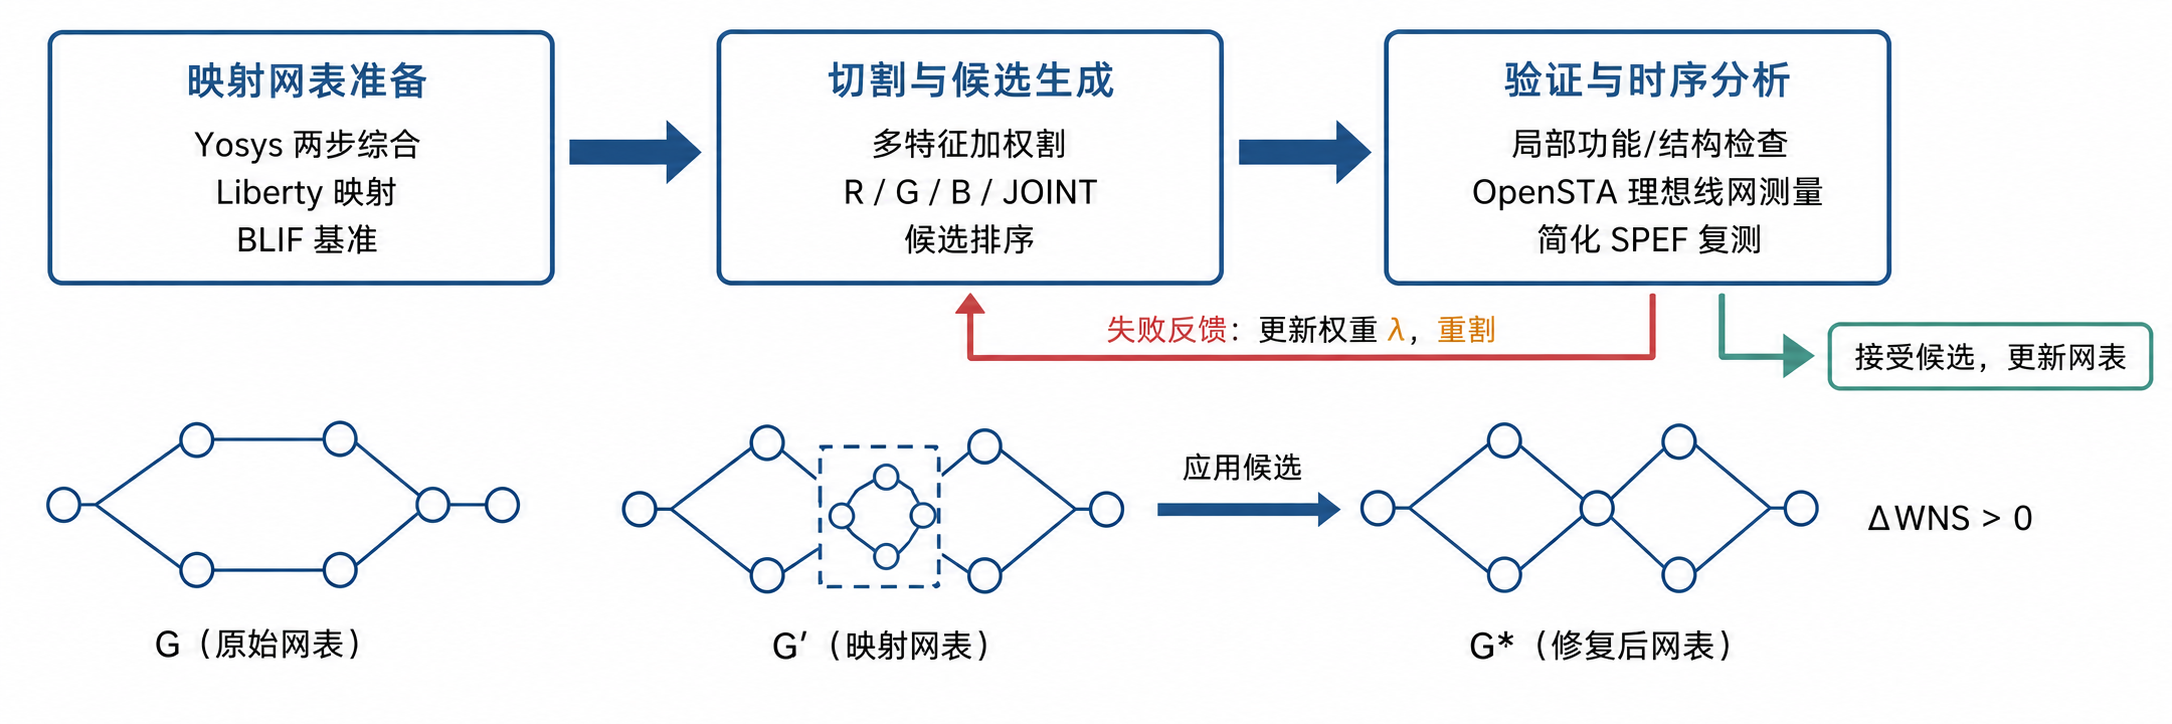
\includegraphics[width=0.96\columnwidth]{fig_method_flow_redraw_20260814.png}%
\caption{FAECO 三阶段流水线：映射网表准备 $\rightarrow$ 切割与候选细化 $\rightarrow$ 验证与时序分析。}
\label{fig:method_flow}
\end{figure}

\begin{algorithm}[H]
\footnotesize
\caption{FAECO 修复流程示意}\label{alg:main}
\begin{algorithmic}[1]
\Require 映射网表 $G'$、时序约束 $T$、工艺库 $\mathcal{L}$
\Ensure 修复后网表 $G^*$、接受候选集合 $\mathcal{A}$
\State 保存基线网表 $G_0\gets G'$，初始化当前网表 $N\gets G_0$、$G^*\gets G_0$、$\mathcal{A}\gets\emptyset$ 和搜索权重 $\lambda$
\Repeat
  \State 从\textbf{当前网表 $N$} 的最差违例端点提取扇入锥，必要时按深度分治
  \State 构建加权割与关键路径覆盖割，生成并排序 R/G/B/JOINT 候选
  \State 对候选执行局部功能/结构检查和 OpenSTA 测量
  \State 对满足物理门控条件的候选进行简化 SPEF 复测
  \State 若候选满足式~\eqref{eq:accept} 并在启用物理门控时通过简化 SPEF 复测，则将其加入 $\mathcal{A}$，并将该候选应用于当前网表、提交为下一轮评估基准（$N\gets N+\Delta$），同时更新最优网表 $G^*$。同一轮内多个候选共享同一基准 $N$ 且互不叠加；该轮一旦提交，基于旧基准的其余候选即作废，下一轮从提交后的网表重新提取违例端点与扇入锥并重新生成候选
  \State \textbf{若启用失效反馈控制}，触发 F1--F6 的失效候选按对应失效类型更新搜索参数；固定权重配置仅记录失效类型、不更新权重。因 10\,ps 阈值直接过滤的候选不参与失效反馈
\Until{无时序违例、候选耗尽或达到停止条件}
\State \Return $G^*,\ \mathcal{A}$
\end{algorithmic}
\end{algorithm}

算法~\ref{alg:main} 给出从违例端点提取扇入锥、生成候选、时序测量到反馈重搜索的流程。候选按轮提交：每轮接受的候选经验证后成为下一轮的评估基准，故多轮配置下修复网表由接受的补丁逐轮累积形成，效率优先配置（\S\ref{sec:eff_prio}）仅执行单轮；候选接受谓词与验证层次在 \S\ref{sec:validation} 中统一定义。算法~\ref{alg:main} 描述候选搜索与提交过程；独立顺序 SEC 在生成最终修复网表后执行，其证明结果单独统计。失效反馈在每轮候选评估结束后按失效类型更新搜索权重，并作用于下一轮的候选构造，不改变当前轮已生成候选的评估顺序；若一轮内候选耗尽且无候选被接受、且尚未达到停止条件，流程更新权重后进入下一轮重新搜索。

\subsection{加权割与候选搜索}\label{sec:mechanism}
\begin{figure*}[!tb]
\centering
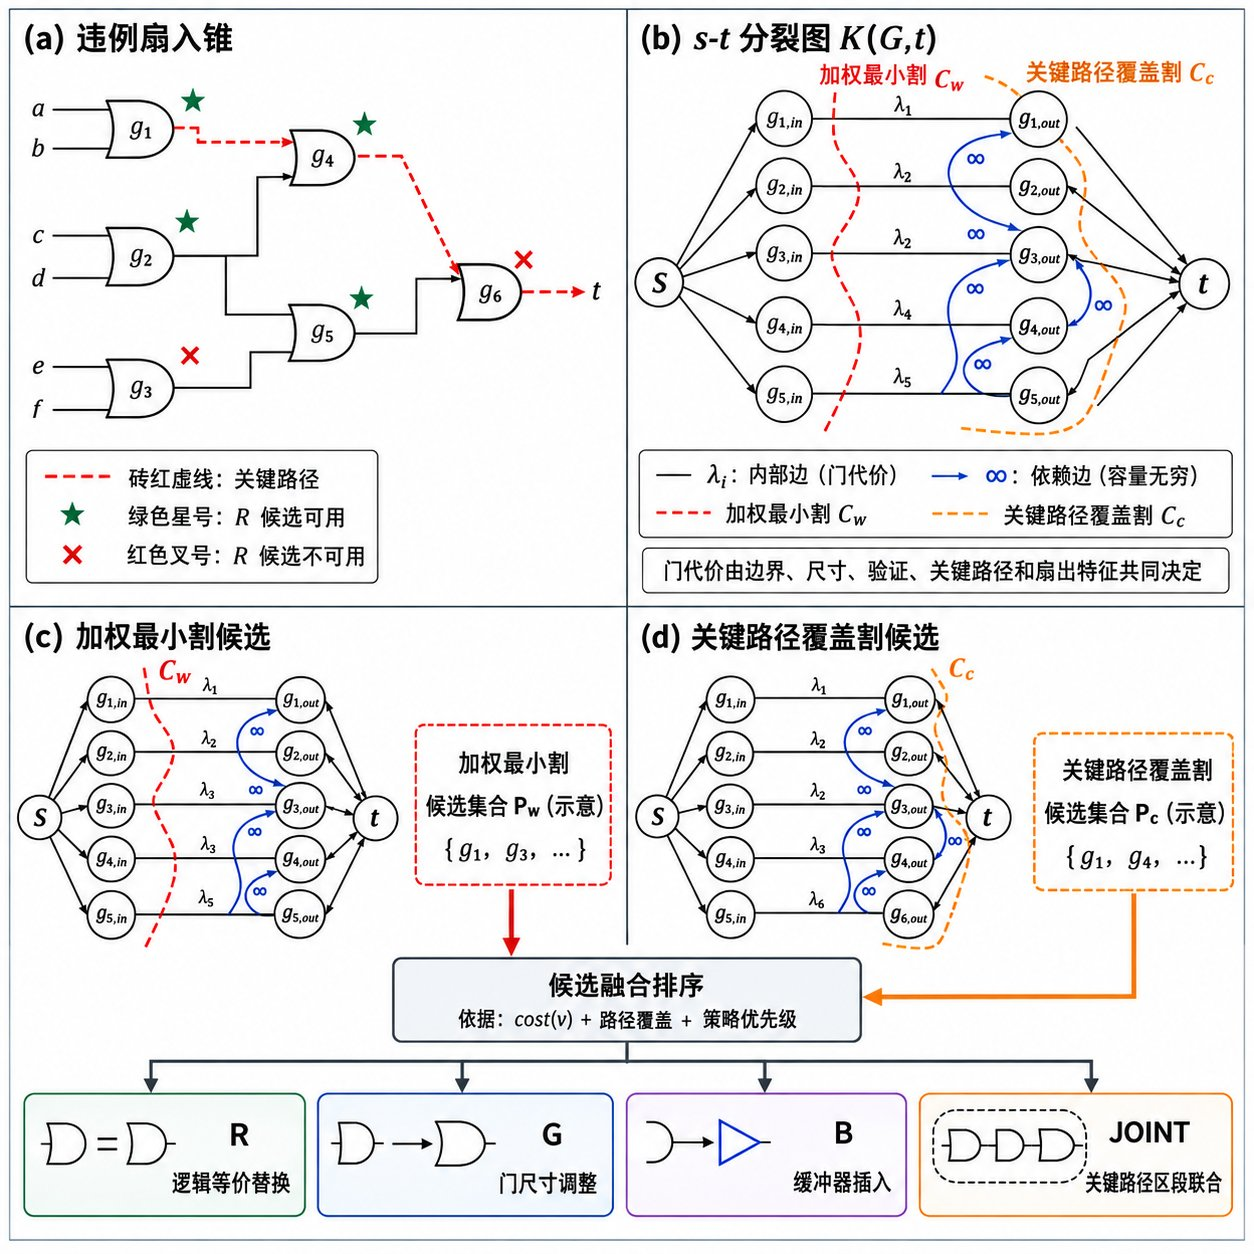
\includegraphics[width=0.65\textwidth]{fig_cut_generation_mechanism_imagegen.png}
\caption{FAECO 候选构造与排序机制：加权最小割控制候选规模，关键路径覆盖割 $C_c$ 补充时序关键候选，R 候选可用性参与策略切换；图中候选集合 $P_w$ 与 $P_c$ 分别对应 $C_w$ 与 $C_c$。}
\label{fig:cut_generation}
\end{figure*}

图~\ref{fig:cut_generation} 展示 FAECO 的主要机制。首先，从违例端点反向提取局部组合扇入锥 $C(G,t)$，并为门节点标注 R 等价候选可用性、关键路径覆盖和候选规模等特征。加权最小割的节点代价由边界、候选规模、验证代价和扇出特征构成，并按权重 $\lambda_c$ 对具备 R 等价候选的门施加深度折扣，如式（2）所示；关键路径覆盖另通过独立的关键路径覆盖割 $C_c$ 形成补充候选，并由 $\lambda_c$ 控制其排序优先级。R 候选的可用性用于候选实例化与策略切换——若某门缺少 R 等价候选，则其关键路径覆盖折扣与扇出代价同时失效并自动转向 G/B 策略。

随后，FAECO 生成两类互补边界：加权最小割 $C_w$ 优先控制局部规模，关键路径覆盖割 $C_c$ 覆盖时序关键门。两类边界分别实例化为 R/G/B/JOINT 候选，统一按割代价、关键路径覆盖和策略优先级排序，交由 OpenSTA 测量 $\Delta_{\mathrm{WNS}}$ 和 $\Delta_{\mathrm{TNS}}$。接受谓词保留有效候选；若启用失效反馈控制，触发 F1--F6 的失效候选按失效类型更新相应搜索权重，作为下一轮候选构造的控制输入。该更新在本文中被定位为\textbf{搜索诊断与控制机制}，其是否带来独立增益由 \S\ref{sec:ablation} 单独检验。

候选 $p$ 的 WNS 改善量在相同 SDC 和时钟约束下定义为：
\begin{equation}\label{eq:dtiming}
\Delta_{\mathrm{WNS}}(p) = \mathrm{WNS}_{\mathrm{after}}(p) - \mathrm{WNS}_{\mathrm{before}}.
\end{equation}
节点代价 $\mathrm{cost}(v)$ 综合边界、尺寸、验证和扇出因素，并按关键路径深度折扣归一化。设 $\mathrm{depth}(v)$ 为 $v$ 在锥内的逻辑深度，$V_R$ 为具备 R 等价候选的门集合，$\mathbb{1}[\cdot]$ 为指示函数，则
{\small
\begin{equation}
\label{eq:cost}
\begin{aligned}
\mathrm{cost}(v) ={}& \Big(1 + \frac{\lambda_b}{1+\mathrm{depth}(v)}
 + \lambda_s\,\frac{s(v)^2}{S_2}
 + 0.01\lambda_v\,n_C \\
 &+ 0.1\lambda_f\,\mathbb{1}[v{\in}V_R]\,\mathrm{fanout}(v)\Big) \\
 &\Big/\Big(1 + \lambda_c\,\mathbb{1}[v{\in}V_R]\,
 \frac{\mathrm{depth}(v)}{\mathrm{depth}_{\max}}\Big),
\end{aligned}
\end{equation}
}
其中 $\lambda_b/\lambda_s/\lambda_v/\lambda_f$ 分别为边界、尺寸、验证和扇出权重，$\lambda_c$ 为关键路径深度折扣权重，默认均为 $1.0$；$n_C=|C(G,t)|$ 为目标扇入锥的门数，$s(v)$ 为门 $v$ 的局部扇入锥规模，$S_2=\sum_u s(u)^2$，$\mathrm{depth}_{\max}=\max_u \mathrm{depth}(u)$。扇出项与分母折扣均以 $\mathbb{1}[v{\in}V_R]$ 为门控：深度折扣与相应扇出项仅作用于存在 R 等价候选的门。对于缺少 R 等价候选的节点，继续施加深度折扣可能使搜索偏向无法实例化为 R 候选的边界，故对此类节点关闭 R 相关折扣，仍允许其参与 G/B 候选生成。$\lambda_c$ 同时参与关键路径覆盖候选的排序，用于调节对高关键度节点的偏好；归一化项用于抑制大锥规模。其中 $0.01$ 和 $0.1$ 为验证规模项与扇出项的固定缩放系数，所有实验均保持不变。

\subsection{特征设计动机}\label{sec:feature_motivation}

式~\eqref{eq:cost} 中的各项特征分别对应预布局门级 ECO 中一类常见的风险。边界特征控制单次改动的区域范围，降低跨越局部逻辑边界候选被优先选择的概率，从而减少后续验证的额外开销；尺寸特征抑制候选局部扇入锥的规模增长，使候选维持在可枚举、可评估的范围内；验证特征按锥内门数施加与验证规模同向的惩罚，使搜索倾向于选择验证规模较小的候选；扇出特征降低高负载节点候选的优先级，以降低引入电气与负载风险的可能；深度特征则提高接近关键路径节点的优先级，使搜索更倾向于覆盖时序关键门。各特征与对应 ECO 风险的对照关系见表~\ref{tab:feature_motivation}。各权重在本文中均取固定值（默认 $1.0$），不随电路与测试集调整。

\begin{table}[ht]
\centering
\caption{加权割特征与对应 ECO 风险的对照}
\label{tab:feature_motivation}
\footnotesize
\setlength{\tabcolsep}{3pt}
\begin{tabular}{>{\raggedright\arraybackslash}p{1.3cm}>{\raggedright\arraybackslash}p{2.6cm}>{\raggedright\arraybackslash}p{3.0cm}}
\toprule
\textbf{特征} & \textbf{式~\eqref{eq:cost} 中的项} & \textbf{对应 ECO 风险与设计取向} \\
\midrule
边界 & 边界惩罚 $\lambda_b/(1+\mathrm{depth})$ & 降低跨越局部逻辑边界候选的优先级 \\
尺寸 & 规模惩罚 $\lambda_s s(v)^2/S_2$ & 控制候选规模，使候选可枚举、可评估 \\
验证 & 验证代价 $0.01\lambda_v n_C$ & 按锥内门数惩罚，倾向选择验证规模较小的候选 \\
扇出 & 扇出惩罚 $0.1\lambda_f\mathrm{fanout}$ & 降低高负载节点候选的优先级 \\
深度 & 深度折扣 $\lambda_c\,\mathrm{depth}/\mathrm{depth}_{\max}$ & 提高关键路径覆盖，优先贴近时序关键门 \\
\bottomrule
\multicolumn{3}{p{0.92\columnwidth}}{\footnotesize 表中各项与式~\eqref{eq:cost} 逐项对应；扇出项与深度折扣均以存在 R 等价候选为门控条件。本表只给出特征的设计取向，不主张权重取值的理论最优性。}\\
\end{tabular}
\end{table}

\subsection{类型化失效刻画与搜索控制}

\FloatBarrier
框架将 F1--F6 定义为六类候选失效，检测条件及对应搜索参数调整见表~\ref{tab:failures}。固定权重配置仅记录失效类型；启用失效反馈控制时，按失效类型调整搜索权重及锥规模上限（每类失效使相应权重增加 $1.0$，F5 额外将最大锥门数减半）。F6 记录简化 SPEF 复测下的物理失效，相关过滤结果见 \S\ref{sec:phys_closure}。本文另实现以指数滑动平均（EMA）平滑的自适应更新，并仅在 \S\ref{sec:ablation} 中作为消融对象。

\begin{table}[!htbp]
\centering
\caption{F1--F6 失效类型与搜索控制动作}
\label{tab:failures}
\scriptsize
\setlength{\tabcolsep}{2pt}
\begin{tabular}{p{2.0cm}p{2.6cm}p{2.9cm}}
\toprule
\textbf{失效类型} & \textbf{检测条件} & \textbf{控制动作} \\
\midrule
F1 局部功能/结构失效 & Liberty 文件中的函数匹配或结构检查未通过 & 增加边界惩罚 $\lambda_b$ 与扇出权重 $\lambda_f$（降低高扇出节点的候选优先级），降低此类节点被选作候选边界的概率 \\
F2 边界失效 & 锥边界未闭合 & 增加边界惩罚 $\lambda_b$，收紧锥边界，保留已映射门 \\
F3 尺寸过大 & 候选尺寸超过阈值 & 增加尺寸惩罚，倾向于选择规模更小的割 \\
F4 时序收益不足 & 候选未满足式~\eqref{eq:accept} & 上调关键路径深度折扣 $\lambda_c$（同时提高覆盖割排序优先级），提高下一轮割集方案中关键路径相关节点的优先级 \\
F5 验证超时 & 局部检查或 STA 运行时间 $>$ 当前配置的单候选验证时限（默认 $60\,$s） & 增加验证代价惩罚 $\lambda_v$ 并将最大锥门数减半 \\
F6 线载估计下的时序失效 & 启用物理门控且理想线网增益 $>10\,$ps，但 SPEF 下 WNS 不改善 & 增加边界惩罚 $\lambda_b$，收紧候选边界并偏向较小局部 \\
\bottomrule
\end{tabular}
\end{table}

\subsection{验证与接受}\label{sec:validation}
FAECO 首先通过局部函数与结构检查筛选候选，再由 OpenSTA 评估时序收益；对于最终修复网表，另行执行独立顺序 SEC。R 候选由 Liberty 函数匹配生成，G/B 候选由保持逻辑函数的局部结构变换生成；组合网表可在启用相应流程时由 ABC \texttt{cec} 回验。主实验和跨测试集实验对最终基线网表与修复网表执行独立顺序 SEC，SEC 结果与理想线网 WNS 候选接受判定分开统计。该 SEC 在 SKY130 行为单元模型下验证组合逻辑与状态转移关系；理想线网 WNS 和 OpenROAD 全局布线寄生估计后的 WNS 分别由 OpenSTA 与 OpenROAD 流程测量。

候选 $p$ 在相同 SDC、时钟约束和分析角下的接受谓词为
\begin{equation}
\label{eq:accept}
\begin{aligned}
\operatorname{Accept}(p)={}&[\Delta_{\mathrm{WNS}}(p)>0]\\
&\lor[\mathrm{tns\_aware}\land\Delta_{\mathrm{WNS}}(p)=0\\
&\qquad\land\Delta_{\mathrm{TNS}}(p)>0].
\end{aligned}
\end{equation}
启用物理门控时，满足式~\eqref{eq:accept} 且理想线网增益超过 10\,ps 的候选进一步接受简化 SPEF 复测；$0<\Delta\mathrm{WNS}\le10\,$ps 的候选不进入最终接受集合。复测下 WNS 仍改善的候选进入接受集合 $\mathcal{A}$，否则记为 F6；启用失效反馈控制时该失效用于下一轮搜索参数更新。未启用物理门控时，SPEF 结果作为独立物理复测，不改变理想线网候选的接受判定。

\subsection{候选构造复杂度}\label{sec:impl}

分裂图采用最大流—最小割求解。若锥内门数为 $n$、扇入依赖边数为 $f$，则分裂图节点数为 $V=2n+2$、边数为 $E=O(n+f)$；采用 Edmonds--Karp 求解时，单次割求解复杂度为 $O(VE^2)$。上述复杂度对应单次最小割求解，不包括候选 STA 测量及最终 SEC 的运行开销；在实际运行中，总运行时间主要由候选级 STA 测量与最终 SEC 决定，单次最小割求解所占比例很小。具体工具版本、运行环境和参数配置见第~\ref{sec:setup} 节。

扇入锥 $C(G, t) = (V_C, E_C)$ 由反向广度优先搜索（BFS）抽取。对大规模设计，按逻辑深度将违例锥切分为受门数上限约束的子锥，独立生成候选并沿关键路径排序，以控制内存和求解规模。

% =============================================================================
% IV. 实验
% =============================================================================
\section{实验}\label{sec:exp}

\subsection{实验设置}\label{sec:setup}

\textbf{环境与数据集}：实验在 WSL2 环境（Ubuntu 24.04.4 LTS，内核 6.6.87.2-microsoft-standard-WSL2）中完成，主机 CPU 为 AMD Ryzen 7 7435H，WSL 可见 16 个逻辑核与 15\,GB 内存；主流程采用 OSS-CAD Suite（Yosys 0.67+146、OpenSTA 3.1.0），顺序 SEC 采用 WSL 环境中的 Yosys 0.33。测试集包含 8 个 ISCAS89、19 个 ITC-99 和 3 个 PicoRV32 子模块，统一采用 0.5 ns 时钟约束以形成时序压力。\textbf{该约束不代表各设计的目标工作频率，实验主要比较相同约束下的 WNS 变化，不等同于时序收敛。}主要评价指标为 WNS、全局布线寄生估计后的 WNS 和候选级 STA 次数；TNS 用于可选的辅助接受判据。本文以 WNS 严格改善作为主要效果统计口径。跨测试集实验中，b06 保留 WNS 持平且 TNS 改善时的辅助接受条件；该类补丁不计入“严格 WNS 改善”统计。其余实验以 WNS 严格改善为主要接受条件；TNS-aware 仅作为可选扩展，不与本文物理门控实验联合启用。

\textbf{基准电路纳入规则}：ISCAS89 纳入能够经统一 Yosys→SKY130 HD 流程成功映射并形成有效 setup timing path 的 8 个顺序电路；ITC-99 按相同标准纳入 19 个电路（b01--b15、b17、b20--b22），其中 b18、b19 未纳入上述统一统计，在相同流程下作为大规模补充实例单独运行并报告（见 \S\ref{sec:itc99}）；PicoRV32 选择主核 \texttt{picorv32}、乘法协处理器 \texttt{picorv32\_pcpi\_mul} 与存储密集子模块 \texttt{picorv32\_regs}（存储簇）以覆盖控制、算术和存储三类结构差异。

\textbf{实验配置}：本文设置单轮修复、跨测试集评估、候选搜索消融及物理验证等实验，各小节结果仅在相同配置内比较。\S\ref{sec:iscas} 采用单轮、首个改善后停止的配置；\S\ref{sec:ood} 采用最多 8 轮的迭代配置；\S\ref{sec:ablation} 在固定的 20 轮预算下比较候选空间与排序策略，并单独检验失效反馈；\S\ref{sec:phys_closure} 评估接受候选的物理估计结果（OpenROAD 后验验证使用 \S\ref{sec:iscas} 的接受候选，SPEF 负载扫描与门控实验单独报告）；\S\ref{sec:s_boundary} 检验结构重综合候选的效果。b17 的验证时限例外见 \S\ref{sec:itc99}。效率优先与 20 轮迭代配置的关键参数对比见表~\ref{tab:configs}。完整脚本和参数随补充材料一同发布。

\begin{table}[!htb]
\centering
\caption{效率优先与 20 轮迭代配置的关键参数对比}
\label{tab:configs}
\scriptsize
\setlength{\tabcolsep}{4pt}
\begin{tabular}{lcc}
\toprule
\textbf{参数} & \textbf{效率优先} & \textbf{20 轮迭代} \\
\midrule
最大迭代轮数                    & 1（首改进即停止） & 20 \\
F1--F6 失效反馈                  & 启用 & 不启用（固定权重） \\
10\,ps 物理门控 SPEF 复测        & 关 & 关 \\
单候选验证时限（默认）           & 60\,s & 60\,s \\
\bottomrule
\multicolumn{3}{p{0.95\columnwidth}}{\footnotesize 注：20 轮迭代配置（\S\ref{sec:ablation}）各列由固定权重运行器产生，用于比较候选空间与候选排序；跨测试集主实验（\S\ref{sec:ood}）最多迭代 8 轮、启用跨轮失效反馈，其余关键参数与效率优先配置相同；效率优先配置虽启用失效反馈，但受单轮上限约束，权重更新不作用于任何候选构造，故其结果与固定权重一致；b17 的验证时限例外（180\,s）属跨测试集实验（\S\ref{sec:itc99}）。}\\
\end{tabular}
\end{table}

\textbf{接受准则}：除 \S\ref{sec:itc99} 所述 b06 的 TNS 辅助接受外，其余主实验均以式~\eqref{eq:accept} 的 WNS 严格改善为主要接受条件。三组测试集在该统一口径下的总体结果见表~\ref{tab:overview}。

\begin{table}[!htb]
\centering
\caption{三个测试集的总体结果（统一迭代配置）}
\label{tab:overview}
\scriptsize
\setlength{\tabcolsep}{3pt}
\begin{tabular}{lcccc}
\toprule
\textbf{测试集} & \textbf{实例数} & \textbf{严格 WNS 改善} & \textbf{$\Delta_{\mathrm{WNS}}$ 均值\,/\,中位 (ns)} & \textbf{SEC 通过} \\
\midrule
ISCAS89  & 8  & 8/8   & 0.16\,/\,0.10 & 8/8 \\
ITC-99   & 19 & 18/19 & 0.43\,/\,0.18 & 18/19 \\
PicoRV32 & 3  & 2/2   & 0.60\,/\,0.60 & 2/2 \\
\bottomrule
\multicolumn{5}{p{0.95\columnwidth}}{\footnotesize 本表为统一跨测试集配置（最多 8 轮迭代、启用跨轮失效反馈）口径；$\Delta_{\mathrm{WNS}}$ 为预布局理想线网下的 WNS 改善量，均值与中位数只在可评估实例上统计。SEC 列为完全证明的修改网表对数；ITC-99 的 b17 有 1 个等价点未完成证明（见 \S\ref{sec:ood}），故记为 18/19。PicoRV32 的 \texttt{picorv32\_regs} 为存储簇、无寄存器到寄存器时序路径，不参与改善判定与统计，其 SEC 不适用。} \\
\end{tabular}
\end{table}

\subsection{单轮 ECO 修复质量与效率}\label{sec:iscas}

图~\ref{fig:iscas_main} 所示的 8 个 ISCAS89 基线网表与修复网表的对比结果，在预布局理想线网模式下经 OpenSTA 测量均实现严格改善；修复候选来自不改写 D 触发器、时钟和复位的 R/G/B/JOINT 构造级保持变换。8 个修复网表均通过独立顺序 SEC（通过率 8/8），证明单元数和时间见表~\ref{tab:sec_iscas8}。接受的候选类型分布为 JOINT 4 个（s27/s382/s420/s953）、G 3 个（s641/s713/s832）、R 1 个（s820）；本组未出现单独接受的 B 候选。\textbf{图~\ref{fig:iscas_main} 对应效率优先配置}\label{sec:eff_prio}，该配置\textbf{不启用 \S\ref{sec:validation} 的 10\,ps 物理门控阈值}，直接以式~\eqref{eq:accept} 的 $\Delta_{\mathrm{WNS}}>0$ 为接受准则，因此 s420 的 +0.01\,ns（10\,ps）接受候选不与 \S\ref{sec:validation} 的过滤规则冲突。

本节与后续多轮实验采用不同的停止条件，结果分别统计。

在本组接受候选上，JOINT 联合多个局部变换，同时调整了局部实现与驱动条件；G 主要改变驱动强度，R 则受工艺库中等价布尔实现的可用性限制。

\begin{figure}[!t]
\centering
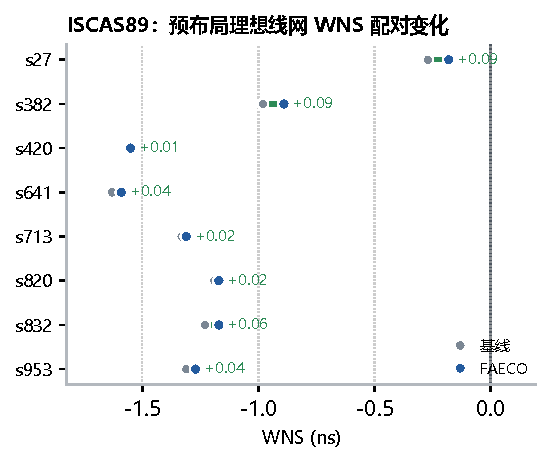
\includegraphics[width=1.0\columnwidth]{fig_iscas89.pdf}
\caption{ISCAS89 顺序电路混合修复的基线与 FAECO 结果对比（周期 0.5 ns；标注为 FAECO 相对基线的 WNS 变化）}
\label{fig:iscas_main}
\end{figure}

\begin{table}[!htb]
\centering
\caption{ISCAS89 顺序门级 SEC 结果}
\label{tab:sec_iscas8}
\setlength{\tabcolsep}{4pt}
\footnotesize
\begin{tabular}{lrrr}
\toprule
\textbf{电路} & \textbf{$\mathrm{equiv}$ 单元} & \textbf{SEC} & \textbf{时间 (s)} \\
\midrule
s27  & 11  & 通过 & 0.303 \\
s382 & 90  & 通过 & 0.382 \\
s420 & 79  & 通过 & 0.368 \\
s641 & 124 & 通过 & 0.381 \\
s713 & 126 & 通过 & 0.410 \\
s820 & 138 & 通过 & 0.454 \\
s832 & 145 & 通过 & 0.437 \\
s953 & 228 & 通过 & 0.537 \\
\bottomrule
\multicolumn{4}{p{0.92\columnwidth}}{\footnotesize 使用 \texttt{equiv\_make} + \texttt{equiv\_simple} + \texttt{equiv\_induct} 进行证明；8 个电路共 8/8 通过。该结果对应 SKY130 行为单元模型下的逻辑门级顺序等价证明。}\\
\end{tabular}
\end{table}

\subsection{跨测试集评估}\label{sec:ood}

\subsubsection{ITC-99 基准族}\label{sec:itc99}

在纳入统一批量评估的 19 个 ITC-99 电路中，18 个电路的 WNS 取得严格改善，b06 与基线持平（$\Delta = 0\,\text{ns}$），19 个电路均无 WNS 回退。b17 在默认 60\,s 单候选验证时限下所有候选均触发 F5 超时而被拒，将其单候选验证时限放宽至 180\,s（其余 18 个电路仍用默认）后，在 104 次候选级 STA 测量内取得 $+0.38\,$ns 改善（接受 G 候选 nor4b$_1\!\to\!$nor4b$_2$）。纳入统计的大规模电路 b14/b15/b17/b20/b21/b22 均取得严格 WNS 改善。b06 的基线 WNS 为 $-0.56\,\text{ns}$，其关键路径包含多个相邻的 \texttt{or4b$_1$} 单元。当前 R/G/B/JOINT 搜索中，G 类替换受到输入电容变化的限制，而 B/R 策略未能形成有效改善；664 次候选级 STA 评估后，未观察到严格 WNS 改善。

接受候选以 G 为主：19 个电路中 17 个含 G 类接受（累计 69 次），B 与 R 类接受分别出现于 14 个和 10 个电路；收益最大的 b20/b21（分别为 $+1.98$ 和 $+2.75\,\text{ns}$）均以 G 为主、辅以 R。19 个电路共进行 3363 次候选级 STA 测量。19 个电路改善量的中位数为 $+0.18\,\text{ns}$、均值为 $+0.43\,\text{ns}$，两者的差异主要来自 b20 和 b21 较大的 WNS 改善幅度（其基线 WNS $\le -13\,\text{ns}$）。各失效类型在 19 个电路上的触发次数见表~\ref{tab:f16_dist}。

作为大规模补充实例（未纳入上述 19 个电路的统一统计）：b18（SKY130 映射后 7.57 万个单元）的 WNS 在 0.5 ns 下由 $-13.34$ ns 改善至 $-13.27$ ns，经 24 次候选级 STA 测量完成修复；b19（15.10 万个单元）由 $-17.44$ ns 改善至 $-16.00$ ns，经 59 次完成。

\subsubsection{PicoRV32 异构族}

基于同一寄存器传输级（RTL）源的三个结构差异明显的子模块直接复用 ISCAS89 流程。其中 PicoRV32 主核与其 PCPI 乘法协处理器 \texttt{picorv32\_pcpi\_mul} 具有有效 setup 路径，分别获得 $+1.13$ 和 $+0.07\,$ns 的改善（修复网表由 R/G/B 多类接受补丁叠加形成）；存储密集子模块 \texttt{picorv32\_regs} 为存储簇、无可建立 setup 路径，因此未执行对应的时序修复，不参与改善判定；该实例未经历时序修复，不属于算法修复失败。

统一跨测试集评估中，三组数据集的 WNS 严格改善比例分别为 8/8、18/19 和 2/2（PicoRV32 中第三个子模块无 setup 路径，不计入分母）。顺序 SEC 面向 30 个测试实例：29 个实例产生实际网表修改，其中 28/29 个修改网表对完全证明（三组分别为 8/8、18/19 和 2/2）；b06 的最终 WNS 与基线持平，其接受的缓冲器/延迟单元补丁不改变 WNS，并经顺序 SEC 完全证明；唯一未产生接受补丁的 \texttt{picorv32\_regs} 无 setup 路径，其输出网表与基线一致。b17 的修复网表经 Yosys \texttt{equiv\_simple} + \texttt{equiv\_induct} 验证 12812 个等价点，另有 1 个等价点未完成证明。该点对应 nor4b$_1\!\to\!$nor4b$_2$ 的同函数尺寸替换，本文将其单独报告。

\subsection{候选空间、排序与反馈消融}\label{sec:ablation}

本节分两组实验。第一组在固定权重及 20 轮迭代预算下比较候选空间与候选评估顺序的联合影响，不单独隔离式~\eqref{eq:cost} 中各特征项的贡献（特征项属候选生成过程的一部分，其权重在本组固定不变）：混合候选策略在 8 个 ISCAS89 电路上的平均 WNS 改善为 1.07\,ns，分别高于纯 G 的 0.16\,ns 和纯 B 的 0.54\,ns。保持混合候选空间不变、随机化评估顺序后，平均改善降至 0.40\,ns。以首次取得改善所需的候选级 STA 次数衡量，候选排序在 7 个有台账的电路中有 6 个少于随机排序的三种子均值，但该指标对随机种子高度敏感——同一电路的不同种子间最大相差 7 倍，且在 s713 上随机排序反而更少（见表~\ref{tab:efficiency}）。因此在本文的实验范围内，候选排序在多数电路上减少了取得首次改善所需的 STA 评估次数，但这一优势并非在所有电路上都成立（各列均为固定搜索权重，见表~\ref{tab:ablation}）。

第二组检验失效反馈的独立作用：保持候选空间、初始权重与候选级 STA 预算（500 次）不变，两配置均采用 20 轮迭代上限并启用提前停止，分别使用固定权重（Fixed）与 EMA 自适应更新（Adaptive）。定义 $B(k)$ 为截至第 $k$ 次候选级 STA 评估的累计最优 WNS 改善（best-so-far 曲线），两种配置在 8 个 ISCAS89 电路上的最终 $\Delta\mathrm{WNS}$、首次改善位置和最大 $B(k)$ 均相同，未观察到 EMA 反馈带来的额外收益。因此，本文不将自适应反馈作为独立的性能提升来源，而把 F1--F6 定位为失效分类及搜索参数调整依据。在第二组的两类配置下，取得相同终点所需的搜索开销见表~\ref{tab:runtime}；表中另列随机排序作为对照。

\begin{table}[H]
\centering
\caption{ISCAS89 候选空间与候选排序设置的 WNS 改善对比（周期 0.5\,ns）}
\label{tab:ablation}
\scriptsize
\setlength{\tabcolsep}{3pt}
\begin{tabular}{lrrrr}
\toprule
\textbf{电路} & \textbf{纯 G} & \textbf{纯 B} & \textbf{随机} & \textbf{混合 20 轮} \\
\midrule
s27  & +0.09 & +0.28 & +0.28 & \textbf{+0.28} \\
s382 & +0.17 & +0.19 & +0.19 & \textbf{+1.00} \\
s420 & +0.35 & +1.00 & +1.15 & \textbf{+1.54} \\
s641 & +0.45 & +1.27 & +0.57 & \textbf{+1.63} \\
s713 & +0.05 & +0.99 & +0.64 & \textbf{+1.33} \\
s820 & +0.02 & +0.26 & +0.15 & \textbf{+0.99} \\
s832 & +0.07 & +0.06 & +0.08 & \textbf{+0.57} \\
s953 & +0.09 & +0.24 & +0.12 & \textbf{+1.25} \\
\midrule
\textbf{均值} & 0.16 & 0.54 & 0.40 & \textbf{1.07} \\
\bottomrule
\multicolumn{5}{p{0.92\columnwidth}}{\footnotesize 数字为 WNS 改善量 (ns)，正值代表修复后 WNS 较基线提高。纯 G / 纯 B 列为单策略候选空间；随机列与混合 20 轮列为混合候选空间，随机列每轮随机化候选评估顺序并取种子 1、2、3 的均值。四列均为固定搜索权重、不启用 F1--F6 权重重整，采用式~\eqref{eq:accept} 与相同的 20 轮上限和候选评估预算，故本表量化候选空间与候选排序的贡献。} \\
\end{tabular}
\end{table}

\begin{table}[!htb]
\centering
\caption{首次取得改善所需的候选级 STA 次数（8 个 ISCAS89 电路，周期 0.5\,ns）}
\label{tab:efficiency}
\scriptsize
\setlength{\tabcolsep}{2pt}
\begin{tabular}{lccccc}
\toprule
\textbf{电路} & \textbf{候选排序} & \multicolumn{3}{c}{\textbf{随机排序}} & \textbf{随机均值} \\
\cmidrule(lr){3-5}
 & & \textbf{种子 1} & \textbf{种子 2} & \textbf{种子 3} & \\
\midrule
s27  & 1 & 3 & 3 & 1 & 2.3 \\
s382 & --- & 6 & 3 & 8 & 5.7 \\
s420 & 2 & 5 & 1 & 1 & 2.3 \\
s641 & 1 & 7 & 5 & 1 & 4.3 \\
s713 & 7 & 1 & 5 & 2 & 2.7 \\
s820 & 1 & 1 & 3 & 1 & 1.7 \\
s832 & 1 & 1 & 2 & 1 & 1.3 \\
s953 & 1 & 3 & 1 & 1 & 1.7 \\
\bottomrule
\multicolumn{6}{p{0.95\columnwidth}}{\footnotesize 数字为整次运行中第一个严格优于基线的候选所处的累积候选序号，即首次取得改善时已消耗的候选级 STA 次数；随机排序列为每轮随机化候选评估顺序的三个独立种子，随机均值为三者的算术平均。候选排序在 7 个有台账的电路中有 6 个少于随机均值（s713 相反），但不同种子间最大相差 7 倍，说明该指标对排序扰动敏感。s382 的候选排序逐候选台账缺失，该格留空。本表与表~\ref{tab:ablation} 同属 20 轮、固定搜索权重配置。} \\
\end{tabular}
\end{table}

\begin{table}[!htb]
\centering
\caption{20 轮迭代配置下的候选级 STA 次数与端到端运行时间（8 个 ISCAS89 电路）}
\label{tab:runtime}
\footnotesize
\setlength{\tabcolsep}{4pt}
\begin{tabular}{>{\raggedright\arraybackslash}p{3.1cm}rr}
\toprule
\textbf{配置} & \textbf{STA 次数} & \textbf{时间 (s)} \\
\midrule
固定权重（候选排序） & 4146 & 2010.8 \\
EMA 自适应 & 4883 & 2065.3 \\
随机排序（三种子均值） & 5624 & 2460.3 \\
\bottomrule
\multicolumn{3}{p{0.92\columnwidth}}{\footnotesize 三行均采用 20 轮迭代上限、提前停止与逐电路候选级 STA 预约上限 500（\texttt{--sta-budget}，在迭代边界检查；随机排序臂在 s420 与 s641 上触及该上限）。表中 STA 次数为 8 个电路候选级 STA 测量次数之和，与上述预约为不同计数口径，故不受 $500\times8$ 约束；时间为各电路墙钟耗时之和（含候选构造、映射与候选级 STA），不计最终 SEC。本表与表~\ref{tab:ablation}、表~\ref{tab:efficiency} 出自不同运行配置，其 STA 计数不与表~\ref{tab:efficiency} 的首次改善位置口径对应。}\\
\end{tabular}
\end{table}


\begin{table}[!htb]
\centering
\caption{F1--F6 失效触发次数（ITC-99 主实验）}
\label{tab:f16_dist}
\scriptsize
\setlength{\tabcolsep}{3pt}
\begin{tabular}{lcccccc}
\toprule
 & \textbf{F1} & \textbf{F2} & \textbf{F3} & \textbf{F4} & \textbf{F5} & \textbf{F6} \\
\midrule
触发次数 & 138 & 3 & 16 & 2434 & 915 & 0 \\
\bottomrule
\multicolumn{7}{p{0.95\columnwidth}}{\footnotesize 统计范围为 19 个 ITC-99 电路、4044 次候选级评估。F4 对应未满足接受判据的候选，占候选级评估的 60.2\%，是本配置下的主导失效类型；F6 只在启用物理门控时触发，本配置未启用，故为 0。} \\
\end{tabular}
\end{table}

\subsection{物理时序评估与失效检测}\label{sec:phys_closure}

本节采用 \S\ref{sec:eff_prio} 效率优先配置的接受候选，与 \S\ref{sec:ablation} 的 20 轮迭代配置分开统计。表~\ref{tab:pr8} 给出了这些接受候选在 OpenROAD 布局及全局布线估计后的时序结果。在 OpenROAD 2.0 布局与全局布线（global routing）寄生估计后，8 个 ISCAS89 电路中有 5 个电路保持时序改善，1 个持平，2 个 WNS 下降（幅度分别为 0.02 ns 和 0.01 ns）。流程使用 OpenROAD 2.0、SKY130 HD 和 0.5 ns 时钟约束。另行开展 SPEF 负载扫描与门控实验，用于观察候选对线载估计的敏感性，并记录 F6 失效。本节的物理结果为基于布局与全局布线寄生估计的后验评估，用于观察接受候选在物理估计下的时序表现，不等同于对物理实现有效性的验证。


独立 SPEF 负载扫描显示，s382 的 R 候选与 b18 的 JOINT 候选的 WNS 改善随估计线长增大而归零，表明线载增大后理想线网 WNS 改善逐步衰减。

\textbf{迭代式门控}：在 40\,$\mu$m/unit 估计线载下（unit 表示一次扇出后沿拓扑/曼哈顿距离累加的相对单位长度），对每条线 $e$ 用简化公式 $L_{\mathrm{est}}(e)=40\,\mu\mathrm{m} \cdot u(e)$、$R_e=r_{\mathrm{unit}}L_{\mathrm{est}}$、$C_e=c_{\mathrm{unit}}L_{\mathrm{est}}$ 估计寄生电阻电容（$r_{\mathrm{unit}}$、$c_{\mathrm{unit}}$ 取自 SKY130 HD \texttt{li1} 层代表 RC），并据此生成简化 SPEF。s382 的 50 个和 b18 的 6 个候选均未通过 SPEF 复测，并被记录为 F6；在启用反馈控制的配置中，相应失效用于更新搜索参数。SPEF 门控能够识别并过滤线载估计下 WNS 收益消失的候选。


\begin{table}[ht]
\centering
\caption{OpenROAD 布局及全局布线寄生估计后的 WNS 对比（8 个 ISCAS89 电路）}
\label{tab:pr8}
\footnotesize
\setlength{\tabcolsep}{2pt}
\begin{tabular}{lrrrrr}
\toprule
 & \multicolumn{2}{c}{\textbf{预布局}} & \multicolumn{2}{c}{\textbf{全局布线估计}} & \\
\cmidrule(lr){2-3}\cmidrule(lr){4-5}
\textbf{电路} & \textbf{基线} & \textbf{修复} & \textbf{基线} & \textbf{修复} & $\Delta$ \\
\midrule
s27  & $-0.27$ & $-0.18$ & $-0.36$ & $-0.22$ & $+0.14$ \\
s382 & $-0.98$ & $-0.89$ & $-1.16$ & $-1.02$ & $+0.14$ \\
s420 & $-1.56$ & $-1.55$ & $-1.80$ & $-1.82$ & $-0.02$ \\
s641 & $-1.63$ & $-1.59$ & $-2.10$ & $-2.02$ & $+0.08$ \\
s713 & $-1.33$ & $-1.31$ & $-1.59$ & $-1.58$ & $+0.01$ \\
s820 & $-1.19$ & $-1.17$ & $-1.52$ & $-1.49$ & $+0.03$ \\
s832 & $-1.23$ & $-1.17$ & $-1.51$ & $-1.51$ & $0.00$ \\
s953 & $-1.31$ & $-1.27$ & $-1.60$ & $-1.61$ & $-0.01$ \\
\bottomrule
\multicolumn{6}{p{0.92\columnwidth}}{\footnotesize 各电路物理估计采用与预布局评估一致的映射网表及接受候选；s27 采用 10\% 利用率布局规划；$\Delta$ 为全局布线寄生估计后修复网表相对基线的 WNS 变化。}\\
\end{tabular}
\end{table}

\subsection{结构候选扩展与能力边界}\label{sec:s_boundary}

除 R/G/B/JOINT 构造级变换外，本文还实现了一类窗口局部结构重综合候选（记为 S），用于评估其是否带来额外的 WNS 改善。为考察候选数量的影响，本文扩大 S 的候选池并做开关对照：关闭 S 后，8 个电路的结果均与原配置一致，两臂的非 S 候选序列一致，候选级 STA 预算未触及上限。结构候选（S）的能力边界见表~\ref{tab:s_boundary}。

\begin{table}[H]
\centering
\caption{结构候选（S）的能力边界}
\label{tab:s_boundary}
\footnotesize
\setlength{\tabcolsep}{8pt}
\begin{tabular}{lrr}
\toprule
\textbf{指标} & \textbf{原配置} & \textbf{扩大候选池} \\
\midrule
S 候选数 & 37 & 126 \\
$\Delta L>0$ & — & 76/126 \\
$\Delta_{\mathrm{WNS}}>0$ & 0 & 0/126 \\
$\Delta_{\mathrm{WNS}}=0$ & — & 36/126 \\
$\Delta_{\mathrm{WNS}}<0$ & — & 90/126 \\
接受电路 & 0/8 & 0/8 \\
\bottomrule
\multicolumn{3}{p{0.9\columnwidth}}{\footnotesize $\Delta L=L_{\mathrm{before}}-L_{\mathrm{after}}$，正值表示 SKY130 映射后逻辑深度降低；$\Delta_{\mathrm{WNS}}=\mathrm{WNS}_{\mathrm{after}}-\mathrm{WNS}_{\mathrm{before}}$，正值表示时序改善。$\Delta L$ 与 $\Delta_{\mathrm{WNS}}$ 为两个相互独立的分类维度，同一候选可同时计入两类，故各行数量不要求相加等于候选总数。}\\
\end{tabular}
\end{table}

扩大候选池后，S 候选数量由 37 增至 126，其中 76 个候选降低了映射后的逻辑深度，但均未取得严格 WNS 改善，另有 90 个候选导致 WNS 下降（其余 36 个 WNS 不变）。结果表明，在当前窗口构造、重综合与映射流程下，扩大候选池并未带来额外 WNS 改善。因此，本文将 S 保留为可选候选类型，不将其计入主要性能贡献。

\section{结论}\label{sec:conclusion}

本文提出面向预布局门级时序 ECO 的 FAECO 框架，通过多特征加权割与关键路径覆盖割构造 R/G/B/JOINT 候选，结合候选失效刻画、迭代提交和分层验证实现局部时序优化。在 ISCAS89、ITC-99 和 PicoRV32 测试集上，分别有 8/8、18/19 和 2/2 个实例取得严格 WNS 改善（PicoRV32 第三个子模块无 setup 路径，不计入分母；仅指 WNS 改善，不等同于时序收敛）。在固定权重、20 轮迭代实验中，混合候选策略的平均 WNS 改善为 1.07\,ns，高于纯 G 策略的 0.16\,ns；随机排序实验进一步表明，候选排序在多数电路上减少了取得首次改善所需的候选级 STA 次数。

消融实验表明，EMA 自适应反馈相较固定权重未取得额外收益，扩展后的 S 候选虽能降低部分电路的逻辑深度，但未带来 WNS 改善。OpenROAD 布局及全局布线估计后，8 个 ISCAS89 电路中有 5 个保持改善、1 个持平、2 个出现不超过 0.02\,ns 的退化。失效统计显示，大部分候选的失败来源于时序收益不足（F4 占候选级评估的 60.2\%），而非功能保持问题，这为后续候选空间设计提供了依据。综上，候选空间与评估顺序是取得时序改善的主要因素（见表~\ref{tab:ablation}）。实验分析进一步揭示了候选排序、验证预算与结构扩展之间的关系，为后续预布局 ECO 搜索策略的设计提供依据。




\renewcommand{\refname}{参考文献}
\ctexset{section = {format=\heiti\fontsize{10.5}{14}\selectfont}}
\footnotesize
\linespread{0.95}\selectfont
\balance
\begin{thebibliography}{99}
\bibitem{ho2010eco} Ho K H, Chen Y P, Fang J W, et al. ECO timing optimization using spare cells and technology remapping[J]. IEEE Transactions on Computer-Aided Design of Integrated Circuits and Systems, 2010, 29(5): 697-710. DOI: 10.1109/TCAD.2010.2043573.
\bibitem{liu2021rlsizer} Lu Y C, Nath S, Khandelwal V, et al. RL-Sizer: VLSI gate sizing for timing optimization using deep reinforcement learning[C] //Proceedings of the 58th ACM/IEEE Design Automation Conference. Piscataway: IEEE, 2021: 733-738. DOI: 10.1109/DAC18074.2021.9586138.
\bibitem{chen2024aito} Wu H, Huang Z, Li X, et al. AiTO: Simultaneous gate sizing and buffer insertion for timing optimization with GNNs and RL[J]. Integration, the VLSI Journal, 2024, 98: 102211. DOI: 10.1016/j.vlsi.2024.102211.
\bibitem{iscas89} Brglez F, Bryan D, Kozminski K. Combinational profiles of sequential benchmark circuits[C] //Proceedings of IEEE International Symposium on Circuits and Systems. Piscataway: IEEE, 1989: 1929-1934. DOI: 10.1109/ISCAS.1989.100747.
\bibitem{itc99} Davidson S. ITC'99 benchmark circuits - preliminary results[C] //Proceedings of IEEE International Test Conference. Piscataway: IEEE, 1999: 1125. DOI: 10.1109/TEST.1999.805857.
\bibitem{kravets2019symbolic} Kravets V N, Lee N Z, Jiang J H R. Comprehensive search for ECO rectification using symbolic sampling[C] //Proceedings of the 56th Annual Design Automation Conference. New York: ACM, 2019: 71:1-71:6. DOI: 10.1145/3316781.3317790.
\bibitem{jiang2010fraig} Wu B H, Yang C J, Huang C Y, et al. A robust functional ECO engine by SAT proof minimization and interpolation techniques[C] //Proceedings of IEEE/ACM International Conference on Computer-Aided Design. Piscataway: IEEE, 2010: 729-734. DOI: 10.5555/2133429.2133584.
\bibitem{jiang2016resource} Cheng A C, Jiang I H R, Jou J Y. Resource-aware functional ECO patch generation[C] //Proceedings of the Design, Automation \& Test in Europe Conference \& Exhibition. Piscataway: IEEE, 2016: 1036-1041. DOI: 10.5555/2971808.2972050.
\bibitem{zhong2024stp} Pan H, Zhang R, Xia Y, et al. A semi-tensor product based circuit simulation for SAT-sweeping[C] //Proceedings of the Design, Automation \& Test in Europe Conference \& Exhibition. Piscataway: IEEE, 2024: 1-6. DOI: 10.23919/DATE58400.2024.10546678.
\bibitem{zhuo2018patch} Dao A Q, Lee N Z, Chen L C, et al. Efficient computation of ECO patch functions[C] //Proceedings of the 55th Annual Design Automation Conference. New York: ACM, 2018: 1-6. DOI: 10.1145/3195970.3196039.
\bibitem{huang2025phys} Ye Y, Xu P, Ren L, et al. Learning-driven physically aware large-scale circuit gate sizing[J]. IEEE Transactions on Computer-Aided Design of Integrated Circuits and Systems, 2025, 44(5): 1901-1914. DOI: 10.1109/TCAD.2024.3488577.
\bibitem{zhang2025buffalo} Hsiao H H, Lu Y C, Lim S K, et al. BUFFALO: PPA-configurable, LLM-based buffer tree generation via group relative policy optimization[C] //Proceedings of IEEE/ACM International Conference on Computer-Aided Design. Piscataway: IEEE, 2025: 1-9. DOI: 10.1109/ICCAD66269.2025.11240744.
\bibitem{openroad} Ajayi T, Chhabria V A, Fogaça M, et al. Toward an open-source digital flow: First learnings from the OpenROAD project[C] //Proceedings of the 56th ACM/IEEE Design Automation Conference. New York: ACM, 2019: 1-4. DOI: 10.1145/3316781.3326334.
\bibitem{abc} Brayton R, Mishchenko A. ABC: An academic industrial-strength verification tool[C] //Proceedings of the 22nd International Conference on Computer Aided Verification. Berlin: Springer, 2010: 24-40. DOI: 10.1007/978-3-642-14295-6\_5.
\end{thebibliography}

\end{document}
